% Preface required in the knitr RnW file
\documentclass{article}\usepackage[]{graphicx}\usepackage[]{color}
%% maxwidth is the original width if it is less than linewidth
%% otherwise use linewidth (to make sure the graphics do not exceed the margin)
\makeatletter
\def\maxwidth{ %
  \ifdim\Gin@nat@width>\linewidth
    \linewidth
  \else
    \Gin@nat@width
  \fi
}
\makeatother

\definecolor{fgcolor}{rgb}{0.345, 0.345, 0.345}
\newcommand{\hlnum}[1]{\textcolor[rgb]{0.686,0.059,0.569}{#1}}%
\newcommand{\hlstr}[1]{\textcolor[rgb]{0.192,0.494,0.8}{#1}}%
\newcommand{\hlcom}[1]{\textcolor[rgb]{0.678,0.584,0.686}{\textit{#1}}}%
\newcommand{\hlopt}[1]{\textcolor[rgb]{0,0,0}{#1}}%
\newcommand{\hlstd}[1]{\textcolor[rgb]{0.345,0.345,0.345}{#1}}%
\newcommand{\hlkwa}[1]{\textcolor[rgb]{0.161,0.373,0.58}{\textbf{#1}}}%
\newcommand{\hlkwb}[1]{\textcolor[rgb]{0.69,0.353,0.396}{#1}}%
\newcommand{\hlkwc}[1]{\textcolor[rgb]{0.333,0.667,0.333}{#1}}%
\newcommand{\hlkwd}[1]{\textcolor[rgb]{0.737,0.353,0.396}{\textbf{#1}}}%
\let\hlipl\hlkwb

\usepackage{framed}
\makeatletter
\newenvironment{kframe}{%
 \def\at@end@of@kframe{}%
 \ifinner\ifhmode%
  \def\at@end@of@kframe{\end{minipage}}%
  \begin{minipage}{\columnwidth}%
 \fi\fi%
 \def\FrameCommand##1{\hskip\@totalleftmargin \hskip-\fboxsep
 \colorbox{shadecolor}{##1}\hskip-\fboxsep
     % There is no \\@totalrightmargin, so:
     \hskip-\linewidth \hskip-\@totalleftmargin \hskip\columnwidth}%
 \MakeFramed {\advance\hsize-\width
   \@totalleftmargin\z@ \linewidth\hsize
   \@setminipage}}%
 {\par\unskip\endMakeFramed%
 \at@end@of@kframe}
\makeatother

\definecolor{shadecolor}{rgb}{.97, .97, .97}
\definecolor{messagecolor}{rgb}{0, 0, 0}
\definecolor{warningcolor}{rgb}{1, 0, 1}
\definecolor{errorcolor}{rgb}{1, 0, 0}
\newenvironment{knitrout}{}{} % an empty environment to be redefined in TeX

\usepackage{alltt}

\usepackage{rotating}
\usepackage{graphics}
\usepackage{latexsym}
\usepackage{color}
\usepackage{listings} % allows for importing code scripts into the tex file
\usepackage{wrapfig}
\usepackage{dcolumn}
\usepackage{placeins}

% Approximately 1 inch borders all around
\setlength\topmargin{-.56in}
\setlength\evensidemargin{0in}
\setlength\oddsidemargin{0in}
\setlength\textwidth{6.49in}
\setlength\textheight{8.6in}

% macros for different spacing options
\makeatletter
\newcommand{\singlespacing}{\let\CS=\@currsize\renewcommand{\baselinestretch}{1}\small\CS}
\newcommand{\doublespacing}{\let\CS=\@currsize\renewcommand{
		\baselinestretch}{1.2}\small\CS}
\newcommand{\normalspacing}{\let\CS=\@currsize\renewcommand{\baselinestretch}{\BLS}\small\CS}
\makeatother

% Options for code listing; from Patrick DeJesus, October 2016
\definecolor{codegreen}{rgb}{0,0.6,0}
\definecolor{codegray}{rgb}{0.5,0.5,0.5}
\definecolor{codepurple}{rgb}{0.58,0,0.82}
\definecolor{backcolour}{rgb}{0.95,0.95,0.92}
\lstdefinestyle{mystyle}{
	backgroundcolor=\color{backcolour},   
	commentstyle=\color{codegreen},
	keywordstyle=\color{magenta},
	numberstyle=\tiny\color{codegray},
	stringstyle=\color{codepurple},
	basicstyle=\footnotesize,
	breakatwhitespace=false,         
	breaklines=true,                 
	captionpos=b,                    
	keepspaces=true,                 
	numbers=left,                    
	numbersep=5pt,                  
	showspaces=false,                
	showstringspaces=false,
	showtabs=false,                  
	tabsize=2
}
%"mystyle" code listing set
\lstset{style=mystyle}
%\lstset{inputpath=appendix/}

\title{Golf Project \\
\large Stat 795}
\author{Aditya, Josh, Kelso}
\date{\today}
\IfFileExists{upquote.sty}{\usepackage{upquote}}{}
\begin{document} 
\maketitle

% Code to start knitr



\doublespacing


\section*{Executive Summary}

%%%%% not done. missing results %%%%

The golf ball manufacturer, Titlest, have claims against smaller companies that some of their brand new balls are not performing to standard. In addition, there is a lawsuit saying that the companies are taking nearly new balls or slightly used balls and either washing or refurbish them, then selling them off as new golf balls. The model of ball in question is ProV1392. 

\section*{Introduction}

In golf, players want to minimize the number of strokes/hits. The best players will have scores or strokes below par. Par is the standard number of strokes needed to make the ball into the hole. In tournaments, players will have negative scores which means that players have repeatedly par. That’s a good thing. In fact, the least amount of stroke made during a game or tournament wins. Tournaments will consistently see negative scores, but a tampered or old ball will affect a player’s game and their number of strokes needed to make the ball.   
The golfing associations which govern the size of golf balls, R\&A and United States Golf Association, specify that the mass of a ball must be no more than 1.620 oz and have a diameter at least 1.680 inches. Any golf balls that do not meet those regulations cannot be used in tournaments. The company Titleist are suing other smaller companies because those smaller companies are washing and refurbishing balls and selling them as new. There are complaints that the ``new" balls are performing below standard. This analysis is to find out if those smaller company is truly washing and refurbishing their balls (ProV1392 model) and selling them as new. 

\section*{Methods}

Hit number is just the observation number. Block is which group the ball is in. Total is the total distance the ball has moved. Carry is the distance from hitting the ball and where it initially lands. Ball model is whether the ball is a new ball, washed ball, or a refurbished ball. C\_ground is the how far the ball rolled after the initial landing of the ball. Traj is the angle which the ball's path has taken. Total dispersion is the distance away from where the ball would have gone if its trajectory was straight or centerline. Ballnum is the id of the ball. 
There were no observations excluded nor included. This analysis is going to use R/RStudio software.

\section*{Results}
\subsection*{Experimental Design}

In order to test to see if there is a difference in performance between brand new golf balls and the washed or refurbished golf balls that are being marketed as new, a well designed experiment must be created. A key element in any well designed experiment is randomization. Care must be taken to ensure that all locations are considered where both the new and refurbished balls are being sold and then a certain amount of both new and refurbished balls be purchased randomly from these locations. The desired sample size is computed from a sample size estimation where 95\% power is achieved for an ANOVA model testing to see if there is a difference between the groups. The sample size chosen for this experiment is 84 observations per group for a total of 252 experimental units. Once the sample has been collected, golf balls will be placed into three separate categories. New golf balls are balls that are actually new and never been used before. Washed golf balls are balls that are used, but simply washing them could get rid of any markings on them. Refurbished balls needed more than a simple washing, and needed to be refinished in order for them to give the appearance of being a new golf ball. Each ball is then placed in a small container and given an unique ball number so that they can be randomly selected during testing.

Once the sample has been collected a series of tests can be conducted to see if there truly is a difference in performance between the new balls and the refurbished balls. We will conduct one test at a time because all that is needed to show that there is, in fact, a difference between the new balls and the refurbished ones is that they perform different in regards to a single metric. The easiest metric to measure is distance, so we will begin by measuring the distance off the tee for each of the groups of golf balls. In order to reduce the amount of error in the model, a machine will swing the golf club to ensure that the golf balls are being struck with a similar amount of force. Multiple measurements will be taken to assess the distance traveled for each ball. Carry distance will measure how far the ball travels in the air and total distance will measure how far the ball travels after it is done rolling. As wind conditions can be a confounding factor in the experiment, a randomized complete block design will be used so that the wind conditions will be similar within each block. Two balls of each kind will be included in each block, and the machine will be recalibrated between blocks to ensure that the force used to hit each ball is consistent. The average golfer swings a golf club at about 93 miles per hour, so this was the swing speed chosen when calibrating the machine.

In addition to the force being used to hit the ball, the trajectory of the ball will have an impact on how far each ball will travel. Due to a variety of different reasons, different golfers hit the ball at different angles. Either they have drivers with different amounts of loft, they place the ball more forward or back in their stance or they fail to make contact with the ball at the optimal point in their swing. For these reasons the trajectory of the ball after impact was altered randomly for each shot and then measured. The trajectory for each shot was randomly chosen from a normal distribution with mean trajectory 4.5 and a standard deviation of 1.5. Since trajectory will have a large effect on the distance traveled, it will need to be included as a covariate in our model. 

\subsection*{Exploratory Data Analysis}

\begin{knitrout}
\definecolor{shadecolor}{rgb}{0.969, 0.969, 0.969}\color{fgcolor}
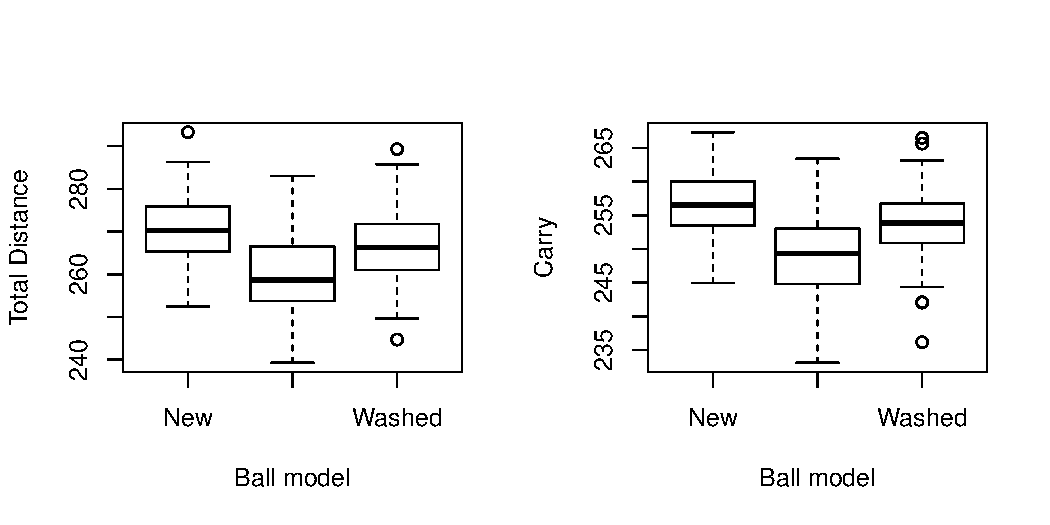
\includegraphics[width=\maxwidth]{figure/box_plots_distance-1} 

\end{knitrout}

\begin{knitrout}
\definecolor{shadecolor}{rgb}{0.969, 0.969, 0.969}\color{fgcolor}
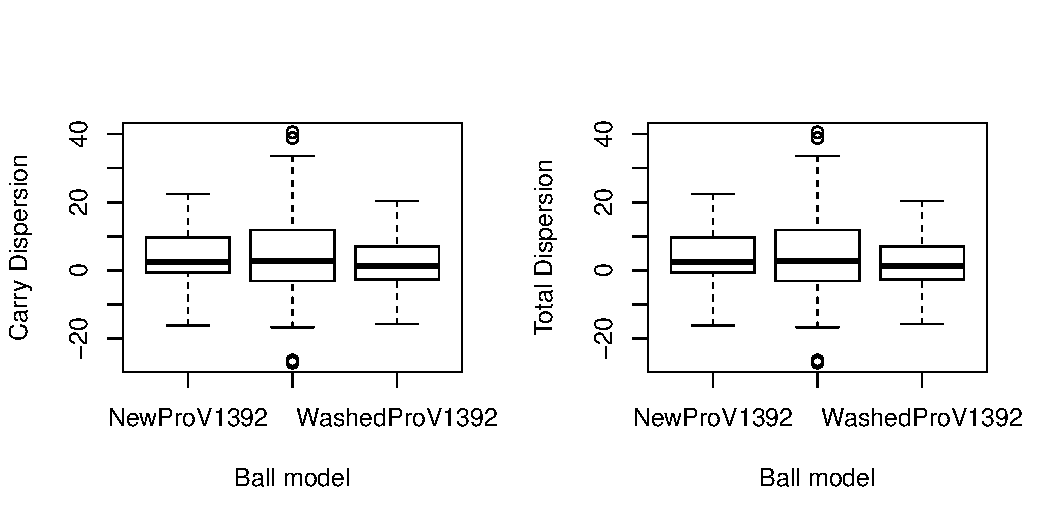
\includegraphics[width=\maxwidth]{figure/box_plots_disp-1} 

\end{knitrout}
From the box plots, it is evident that the carry distance and total distance is considerably high for new balls compared to washed and refurbished balls. Washed balls have a higher carry and total distance compared to the refurbished balls. Total dispersion and carry dispersion is almost same for new and refurbished balls whereas it is slightly less for washed balls as compared to new and refurbished balls.

Trajectory, which is considered as a covariate has a high negative correlation with carry and total distance which seems logical.

\subsection*{Model Selection/Inferences}
We are concerned about the total distance travelled by the ``new" balls. Since a controlled experiment was conducted, we have controlled blocks and treatement. Ball model is the treatment effect and block is the block effect. Trajectory which is a continuous variable is considered as covariate. Analysis of covariance model is selected since our explanatory variables are a mix of categorical and continuous variables.

A linear relationship between the dependent variable and covariate is essential for a ANCOVA analysis. We plot the carry distance against the trajectory to check the linear relationship between them.

\begin{figure}[ht]
\centering
\begin{knitrout}
\definecolor{shadecolor}{rgb}{0.969, 0.969, 0.969}\color{fgcolor}
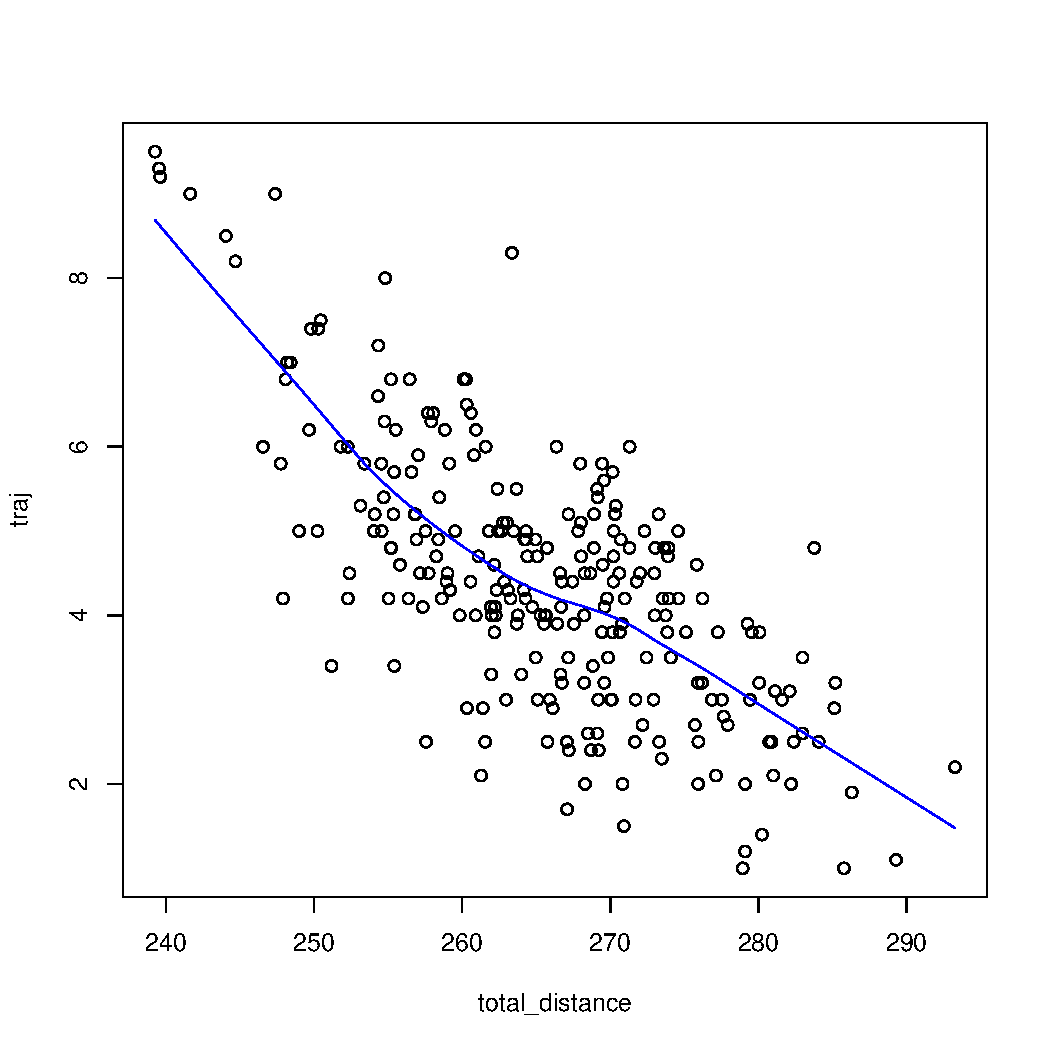
\includegraphics[width=\maxwidth]{figure/linearity_of_variables-1} 

\end{knitrout}
\caption{Relationship between Carry Distance and Trajectory}
\label{Relationship between covariate and Response}
\end{figure}
The red line indicates the linear fit and the blue curve indicates the fit obtained from lowess smoothing. Since both of the lines are very close to each other, we can consider the relationship between carry distance and trajectory as linear. Hence we can proceed with the Analysis of Covariance model.


\subsection*{Analysis of Covariance}

Since we are concerned about the impact of the covariate, black and treatment on the distance, we check the distance till the first impact, carry distance. An ANCOVA analysis was performed, where impact of covariate trajectory, block and ball model on the carry distance was performed. Since we want to identify the effects for trajectory, ballmodel and block when the effects for the others were adjusted, we use type III sum of squares. The type III sum of square methods evaluates the contribution of each factor after considering the contributions of all the other factors/effects in the model.



The ANCOVA table is as follows

\begin{table}[ht]
\centering
\begin{tabular}{|l|rrrr|}
  \hline
 & Sum Sq & Df & F value & Pr($>$F) \\ 
  \hline
(Intercept) & 330057.10 & 1 & 39346.39 & 0.0000 \\ 
  Trajectory & 740.82 & 1 & 88.31 & 0.0000 \\ 
  Block & 2637.49 & 41 & 7.67 & 0.0000 \\ 
  BallModel & 770.36 & 2 & 45.92 & 0.0000 \\ 
  Residuals & 1736.42 & 207 &  &  \\ 
   \hline
\end{tabular}
\caption{ANCOVA table for Carry Distance}
\end{table}

\bigskip

\bigskip

Trajectory, Ball model and block has a significant effect on the carry distance of the ball. Similarly there is a significant impact of Trajectory, Ball model and block on total distance. However, when carry dispersion and total dispersion was considered as the response variable, there was no significant effect of trajectory and ball model but only significant effect of blocks. This is not surprising as there are different terrain and wind conditions in different blocks.

\subsection*{Model Diagnostics}

Dignostic plots help us identify if the residuals deviates from the distributional assumptions and if there is any outlier and influential point.  

\begin{knitrout}
\definecolor{shadecolor}{rgb}{0.969, 0.969, 0.969}\color{fgcolor}
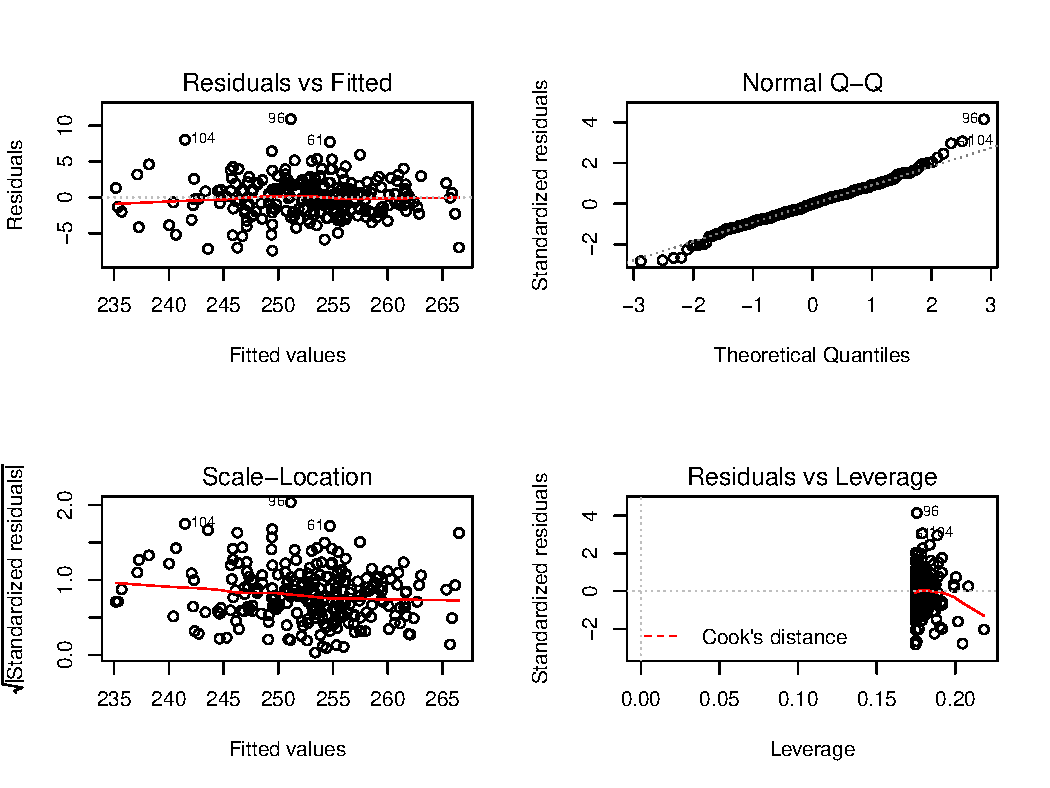
\includegraphics[width=\maxwidth]{figure/diagnostics-1} 

\end{knitrout}
The Residuals vs. Fitted plot indicates that the errors have a constant variance as there is no visible pattern for the residuals and the line is roughly horizontal around 0. Normal Q-Q plot indicates the points are close to the line except for a couple of deviations at either ends of line. Thus, the normality assumption of residuals is satisfied. Scale location plot indicates residuals are randomly spread accross the range of predictors. Hence the homoscedasticity assumption of residuals is satisfied. In the Residuals vs. Leverage plot, there is no point with high Cook's distance score. That is no outlying values present beyond the Cook's distance cutoff line on the upper right corner and lower right corner which means there is no influential point in the dataset. Since all the distributional assumptions of residuals are satisfied, we can consider our model to be a good model.
\section*{Conclusion}
There is a significant effect of covariate trajectory, block and treatment which is the ball models. Hence the golf ball manufacturer, Titlest's claim against the smaller companies is valid. Since the design was controlled with various block effects, the performance was tested in sufficiently large number of conditions and the evidence obtained from the analysis holds in good shape.


\newpage
\noindent {{\bf Appendix }}

The ANCOVA table when total distance is considered as the response variable is as follows

\begin{table}[ht]
\centering
\begin{tabular}{|l|rrrr|}
  \hline
 & Sum Sq & Df & F value & Pr($>$F) \\ 
  \hline
(Intercept) & 379839 & 1 & 15376.2874 & 0.0000 \\ 
  Trajectory & 1810 & 1 & 73.2638 & 0.0000 \\ 
  Block & 6133 & 41 & 6.0551 & 0.0000 \\ 
  BallModel & 1526 & 2 & 30.8796 & 0.0000 \\ 
  Residuals & 5114 & 207 &  &  \\ 
   \hline
\end{tabular}
\caption{ANCOVA table for Total Distance}
\end{table}


The ANCOVA table when total dispersion is considered as the response variable is as follows




\begin{table}[ht]
\centering
\begin{tabular}{|l|rrrr|}
  \hline
 & Sum Sq & Df & F value & Pr($>$F) \\ 
  \hline
(Intercept) & 11.2 & 1 & 0.1382 & 0.71046 \\ 
  Trajectory & 299.1 & 1 & 3.6963 & 0.05591 \\ 
  Block & 4846.2 & 41 & 1.4610 & 0.04611 \\ 
  BallModel & 418.3 & 2 & 2.549 & 0.07784 \\ 
  Residuals & 16747.6 & 207 &  &  \\ 
   \hline
\end{tabular}
\caption{ANCOVA table for Total Dispersion}
\end{table}

The ANCOVA table when carry dispersion is considered as the response variable is as follows

\begin{table}[ht]
\centering
\begin{tabular}{|l|rrrr|}
  \hline
 & Sum Sq & Df & F value & Pr($>$F) \\ 
  \hline
(Intercept) & 0.5 & 1 & 0.0088 & 0.92545 \\ 
  Trajectory & 165.6 & 1 & 2.7057 & 0.10150 \\ 
  Block & 3823.8 & 41 & 1.5242 & 0.03046 \\ 
  BallModel & 279.4 & 2 & 2.2827 & 0.10457 \\ 
  Residuals & 12666.2 & 207 &  &  \\ 
   \hline
\end{tabular}
\caption{ANCOVA table for Carry Dispersion}
\end{table}


\end{document}
